%% bare_conf.tex
%% V1.4b
%% 2015/08/26
%% by Michael Shell
%% See:
%% http://www.michaelshell.org/
%% for current contact information.
%%
%% This is a skeleton file demonstrating the use of IEEEtran.cls
%% (requires IEEEtran.cls version 1.8b or later) with an IEEE
%% conference paper.
%%
%% Support sites:
%% http://www.michaelshell.org/tex/ieeetran/
%% http://www.ctan.org/pkg/ieeetran
%% and
%% http://www.ieee.org/

%%*************************************************************************
%% Legal Notice:
%% This code is offered as-is without any warranty either expressed or
%% implied; without even the implied warranty of MERCHANTABILITY or
%% FITNESS FOR A PARTICULAR PURPOSE! 
%% User assumes all risk.
%% In no event shall the IEEE or any contributor to this code be liable for
%% any damages or losses, including, but not limited to, incidental,
%% consequential, or any other damages, resulting from the use or misuse
%% of any information contained here.
%%
%% All comments are the opinions of their respective authors and are not
%% necessarily endorsed by the IEEE.
%%
%% This work is distributed under the LaTeX Project Public License (LPPL)
%% ( http://www.latex-project.org/ ) version 1.3, and may be freely used,
%% distributed and modified. A copy of the LPPL, version 1.3, is included
%% in the base LaTeX documentation of all distributions of LaTeX released
%% 2003/12/01 or later.
%% Retain all contribution notices and credits.
%% ** Modified files should be clearly indicated as such, including  **
%% ** renaming them and changing author support contact information. **
%%*************************************************************************

% *** Authors should verify (and, if needed, correct) their LaTeX system  ***
% *** with the testflow diagnostic prior to trusting their LaTeX platform ***
% *** with production work. The IEEE's font choices and paper sizes can   ***
% *** trigger bugs that do not appear when using other class files.       ***                          ***
% The testflow support page is at:
% http://www.michaelshell.org/tex/testflow/

\documentclass[journal]{IEEEtran}
% Some Computer Society conferences also require the compsoc mode option,
% but others use the standard conference format.
%
% If IEEEtran.cls has not been installed into the LaTeX system files,
% manually specify the path to it like:
% \documentclass[conference]{../sty/IEEEtran}

% Some very useful LaTeX packages include:
% (uncomment the ones you want to load)

% *** MISC UTILITY PACKAGES ***
%
%\usepackage{ifpdf}
% Heiko Oberdiek's ifpdf.sty is very useful if you need conditional
% compilation based on whether the output is pdf or dvi.
% usage:
% \ifpdf
%   % pdf code
% \else
%   % dvi code
% \fi
% The latest version of ifpdf.sty can be obtained from:
% http://www.ctan.org/pkg/ifpdf
% Also, note that IEEEtran.cls V1.7 and later provides a builtin
% \ifCLASSINFOpdf conditional that works the same way.
% When switching from latex to pdflatex and vice-versa, the compiler may
% have to be run twice to clear warning/error messages.

% *** CITATION PACKAGES ***
%
\usepackage{cite}
% cite.sty was written by Donald Arseneau
% V1.6 and later of IEEEtran pre-defines the format of the cite.sty package
% \cite{} output to follow that of the IEEE. Loading the cite package will
% result in citation numbers being automatically sorted and properly
% "compressed/ranged". e.g., [1], [9], [2], [7], [5], [6] without using
% cite.sty will become [1], [2], [5]--[7], [9] using cite.sty. cite.sty's
% \cite will automatically add leading space, if needed. Use cite.sty's
% noadjust option (cite.sty V3.8 and later) if you want to turn this off
% such as if a citation ever needs to be enclosed in parenthesis.
% cite.sty is already installed on most LaTeX systems. Be sure and use
% version 5.0 (2009-03-20) and later if using hyperref.sty.
% The latest version can be obtained at:
% http://www.ctan.org/pkg/cite
% The documentation is contained in the cite.sty file itself.

% *** GRAPHICS RELATED PACKAGES ***
%
\ifCLASSINFOpdf
  \usepackage[pdftex]{graphicx}
  % declare the path(s) where your graphic files are
  % \graphicspath{{../pdf/}{../jpeg/}}
  % and their extensions so you won't have to specify these with
  % every instance of \includegraphics
  % \DeclareGraphicsExtensions{.pdf,.jpeg,.png}
\else
  % or other class option (dvipsone, dvipdf, if not using dvips). graphicx
  % will default to the driver specified in the system graphics.cfg if no
  % driver is specified.
  \usepackage[dvips]{graphicx}
  % declare the path(s) where your graphic files are
  % \graphicspath{{../eps/}}
  % and their extensions so you won't have to specify these with
  % every instance of \includegraphics
  % \DeclareGraphicsExtensions{.eps}
\fi
% graphicx was written by David Carlisle and Sebastian Rahtz. It is
% required if you want graphics, photos, etc. graphicx.sty is already
% installed on most LaTeX systems. The latest version and documentation
% can be obtained at: 
% http://www.ctan.org/pkg/graphicx
% Another good source of documentation is "Using Imported Graphics in
% LaTeX2e" by Keith Reckdahl which can be found at:
% http://www.ctan.org/pkg/epslatex
%
% latex, and pdflatex in dvi mode, support graphics in encapsulated
% postscript (.eps) format. pdflatex in pdf mode supports graphics
% in .pdf, .jpeg, .png and .mps (metapost) formats. Users should ensure
% that all non-photo figures use a vector format (.eps, .pdf, .mps) and
% not a bitmapped formats (.jpeg, .png). The IEEE frowns on bitmapped formats
% which can result in "jaggedy"/blurry rendering of lines and letters as
% well as large increases in file sizes.
%
% You can find documentation about the pdfTeX application at:
% http://www.tug.org/applications/pdftex

% *** MATH PACKAGES ***
%
\usepackage{amsmath}
% A popular package from the American Mathematical Society that provides
% many useful and powerful commands for dealing with mathematics.
%
% Note that the amsmath package sets \interdisplaylinepenalty to 10000
% thus preventing page breaks from occurring within multiline equations. Use:
%\interdisplaylinepenalty=2500
% after loading amsmath to restore such page breaks as IEEEtran.cls normally
% does. amsmath.sty is already installed on most LaTeX systems. The latest
% version and documentation can be obtained at:
% http://www.ctan.org/pkg/amsmath

% *** SPECIALIZED LIST PACKAGES ***
%
%\usepackage{algorithmic}
% algorithmic.sty was written by Peter Williams and Rogerio Brito.
% This package provides an algorithmic environment fo describing algorithms.
% You can use the algorithmic environment in-text or within a figure
% environment to provide for a floating algorithm. Do NOT use the algorithm
% floating environment provided by algorithm.sty (by the same authors) or
% algorithm2e.sty (by Christophe Fiorio) as the IEEE does not use dedicated
% algorithm float types and packages that provide these will not provide
% correct IEEE style captions. The latest version and documentation of
% algorithmic.sty can be obtained at:
% http://www.ctan.org/pkg/algorithms
% Also of interest may be the (relatively newer and more customizable)
% algorithmicx.sty package by Szasz Janos:
% http://www.ctan.org/pkg/algorithmicx

% *** ALIGNMENT PACKAGES ***
%
%\usepackage{array}
% Frank Mittelbach's and David Carlisle's array.sty patches and improves
% the standard LaTeX2e array and tabular environments to provide better
% appearance and additional user controls. As the default LaTeX2e table
% generation code is lacking to the point of almost being broken with
% respect to the quality of the end results, all users are strongly
% advised to use an enhanced (at the very least that provided by array.sty)
% set of table tools. array.sty is already installed on most systems. The
% latest version and documentation can be obtained at:
% http://www.ctan.org/pkg/array

% IEEEtran contains the IEEEeqnarray family of commands that can be used to
% generate multiline equations as well as matrices, tables, etc., of high
% quality.

\usepackage{booktabs}
\usepackage{multirow}
\usepackage{tabularx}
\usepackage[l3]{csvsimple}

% *** SUBFIGURE PACKAGES ***
%\ifCLASSOPTIONcompsoc
%  \usepackage[caption=false,font=normalsize,labelfont=sf,textfont=sf]{subfig}
%\else
%  \usepackage[caption=false,font=footnotesize]{subfig}
%\fi
% subfig.sty, written by Steven Douglas Cochran, is the modern replacement
% for subfigure.sty, the latter of which is no longer maintained and is
% incompatible with some LaTeX packages including fixltx2e. However,
% subfig.sty requires and automatically loads Axel Sommerfeldt's caption.sty
% which will override IEEEtran.cls' handling of captions and this will result
% in non-IEEE style figure/table captions. To prevent this problem, be sure
% and invoke subfig.sty's "caption=false" package option (available since
% subfig.sty version 1.3, 2005/06/28) as this is will preserve IEEEtran.cls
% handling of captions.
% Note that the Computer Society format requires a larger sans serif font
% than the serif footnote size font used in traditional IEEE formatting
% and thus the need to invoke different subfig.sty package options depending
% on whether compsoc mode has been enabled.
%
% The latest version and documentation of subfig.sty can be obtained at:
% http://www.ctan.org/pkg/subfig

% *** FLOAT PACKAGES ***
%
%\usepackage{fixltx2e}
% fixltx2e, the successor to the earlier fix2col.sty, was written by
% Frank Mittelbach and David Carlisle. This package corrects a few problems
% in the LaTeX2e kernel, the most notable of which is that in current
% LaTeX2e releases, the ordering of single and double column floats is not
% guaranteed to be preserved. Thus, an unpatched LaTeX2e can allow a
% single column figure to be placed prior to an earlier double column
% figure.
% Be aware that LaTeX2e kernels dated 2015 and later have fixltx2e.sty's
% corrections already built into the system in which case a warning will
% be issued if an attempt is made to load fixltx2e.sty as it is no longer
% needed.
% The latest version and documentation can be found at:
% http://www.ctan.org/pkg/fixltx2e

%\usepackage{stfloats}
% stfloats.sty was written by Sigitas Tolusis. This package gives LaTeX2e
% the ability to do double column floats at the bottom of the page as well
% as the top. (e.g., "\begin{figure*}[!b]" is not normally possible in
% LaTeX2e). It also provides a command:
%\fnbelowfloat
% to enable the placement of footnotes below bottom floats (the standard
% LaTeX2e kernel puts them above bottom floats). This is an invasive package
% which rewrites many portions of the LaTeX2e float routines. It may not work
% with other packages that modify the LaTeX2e float routines. The latest
% version and documentation can be obtained at:
% http://www.ctan.org/pkg/stfloats
% Do not use the stfloats baselinefloat ability as the IEEE does not allow
% \baselineskip to stretch. Authors submitting work to the IEEE should note
% that the IEEE rarely uses double column equations and that authors should try
% to avoid such use. Do not be tempted to use the cuted.sty or midfloat.sty
% packages (also by Sigitas Tolusis) as the IEEE does not format its papers in
% such ways.
% Do not attempt to use stfloats with fixltx2e as they are incompatible.
% Instead, use Morten Hogholm'a dblfloatfix which combines the features
% of both fixltx2e and stfloats:
%
% \usepackage{dblfloatfix}
% The latest version can be found at:
% http://www.ctan.org/pkg/dblfloatfix

% *** PDF, URL AND HYPERLINK PACKAGES ***
%
\usepackage{url}
\usepackage{hyperref}
% url.sty was written by Donald Arseneau. It provides better support for
% handling and breaking URLs. url.sty is already installed on most LaTeX
% systems. The latest version and documentation can be obtained at:
% http://www.ctan.org/pkg/url
% Basically, \url{my_url_here}.

% *** Do not adjust lengths that control margins, column widths, etc. ***
% *** Do not use packages that alter fonts (such as pslatex).         ***
% There should be no need to do such things with IEEEtran.cls V1.6 and later.
% (Unless specifically asked to do so by the journal or conference you plan
% to submit to, of course. )

% correct bad hyphenation here
\hyphenation{op-tical net-works semi-conduc-tor}

\begin{document}
%
% paper title
% Titles are generally capitalized except for words such as a, an, and, as,
% at, but, by, for, in, nor, of, on, or, the, to and up, which are usually
% not capitalized unless they are the first or last word of the title.
% Linebreaks \\ can be used within to get better formatting as desired.
% Do not put math or special symbols in the title.
\title{Acoustic Is All You Need: Recognize Alzheimer's Dementia Using Speech Only}

% author names and affiliations
% use a multiple column layout for up to three different
% affiliations
\author{Chun-Mu Weng, Chen-Chun Wu, Jericho Jacques Michael Fajardo, Shun-Han Chang, Tai-Hsiang Peng and Ting-Yu Lin}

% conference papers do not typically use \thanks and this command
% is locked out in conference mode. If really needed, such as for
% the acknowledgment of grants, issue a \IEEEoverridecommandlockouts
% after \documentclass

% for over three affiliations, or if they all won't fit within the width
% of the page, use this alternative format:
% 
%\author{\IEEEauthorblockN{Michael Shell\IEEEauthorrefmark{1},
%Homer Simpson\IEEEauthorrefmark{2},
%James Kirk\IEEEauthorrefmark{3}, 
%Montgomery Scott\IEEEauthorrefmark{3} and
%Eldon Tyrell\IEEEauthorrefmark{4}}
%\IEEEauthorblockA{\IEEEauthorrefmark{1}School of Electrical and Computer Engineering\\
%Georgia Institute of Technology,
%Atlanta, Georgia 30332--0250\\ Email: see http://www.michaelshell.org/contact.html}
%\IEEEauthorblockA{\IEEEauthorrefmark{2}Twentieth Century Fox, Springfield, USA\\
%Email: homer@thesimpsons.com}
%\IEEEauthorblockA{\IEEEauthorrefmark{3}Starfleet Academy, San Francisco, California 96678-2391\\
%Telephone: (800) 555--1212, Fax: (888) 555--1212}
%\IEEEauthorblockA{\IEEEauthorrefmark{4}Tyrell Inc., 123 Replicant Street, Los Angeles, California 90210--4321}}

% use for special paper notices
%\IEEEspecialpapernotice{(Invited Paper)}

% The paper headers
\markboth{Introduction to Machine Learning}%
{Team 39: Acoustic Is All You Need}
% The only time the second header will appear is for the odd numbered pages
% after the title page when using the twoside option.
% 
% *** Note that you probably will NOT want to include the author's ***
% *** name in the headers of peer review papers.                   ***
% You can use \ifCLASSOPTIONpeerreview for conditional compilation here if
% you desire.

% make the title area
\maketitle

% As a general rule, do not put math, special symbols or citations
% in the abstract
\begin{abstract}
Leveraging the most state-of-the-art, cutting-edge transformers, we have beat the baseline and outperformed other teams with acoustic features alone in the classification task of ADReSS\textsubscript{o} challenge at INTERSPEECH 2021. Our groundbreaking results revealed a remarkable insight that acoustic features suffice indeed.
\end{abstract}

% no keywords

\begin{IEEEkeywords}
Alzheimer's disease, machine learning, deep learning, transformer, audio classification.
\end{IEEEkeywords}

% For peer review papers, you can put extra information on the cover
% page as needed:
% \ifCLASSOPTIONpeerreview
% \begin{center} \bfseries EDICS Category: 3-BBND \end{center}
% \fi
%
% For peerreview papers, this IEEEtran command inserts a page break and
% creates the second title. It will be ignored for other modes.
\IEEEpeerreviewmaketitle

\section{Introduction}
% no \IEEEPARstart
Alzheimer's disease (AD) is a neurodegenerative disorder. Traditional methods for monitoring dementia progression include cognitive tests like the Mini-Mental State Examination (MMSE)\cite{MMSE} and the Montreal Cognitive Assessment (MoCA). Although these assessments are widely used, detecting dementia in its early stages, particularly in mild cases, presents a significant challenge. To tackle this issue, voice technology has emerged as a potential solution in aiding early detection systems.

In the field of machine learning, audio analysis shows great promise. The influence of AD on speech involves linguistic aspects such as speech rhythm patterns, disfluencies, and speech quality, as well as language-related elements like vocabulary selection and grammar usage. In this context, we will introduce the ADReSS\textsubscript{o} 2021 Interspeech Challenge, a competition focused on analyzing Alzheimer's disease data through speech recognition.

\subsection{The Challenges}

DementiaBank\cite{weiss2012dementiabank}, a part of TalkBank, curates an extensive and diverse repository of multimedia and corpora for the study of dementia. Moreover, it features several challenges, such as ADReSS 2020 INTERSPEECH challenge, ADReSS\textsubscript{o} 2021 INTERSPEECH challenge and ADReSS-M 2023 ICASSP challenge.

All three challenges have a commonality of participants being asked to describe the situation based on the ``cookie-theft'' picture from the Boston Diagnostic Aphasia Exam\cite{BADE}. The main difference between the ADReSS challenge and the rest is the provision of linguistic data; specifically, ADReSS offered transcripts, while the other challenges did not. On the other hand, the spike in difficulty of the ADReSS-M challenge is its multilingual nature. Unlike the other challenges with English training and testing data, ADReSS-M adopted Greek testing data despite using English training data.

\subsection{The ADReSS\textsubscript{o} Challenge and Dataset}

Regarding the ADReSS-M 2023 ICASSP Challenge which involves a cross-lingual test between English and Greek, we found that the accuracy of the results was unsatisfactory after experimentation. This is the reason why we have decided to primarily focus on the ADReSS\textsubscript{o} 2021 INTERSPEECH Challenge instead.

The ADReSS\textsubscript{o} 2021 INTERSPEECH Challenge training datasets consist of 166 spontaneous recordings (87 with AD, 79 without AD), whereas the testing datasets consist of 71 recordings (35 with AD, 36 without AD). The entirety of the recordings focus on the English version of the ``cookie theft'' challenge with each having an average length of 77.56 seconds and a standard deviation of 38.72 seconds.

In this work, we present the results and analysis of the submissions to the ADReSS\textsubscript{o} challenge.

\section{Literature Review}

There were a total of 12 proceedings in the ADReSS\textsubscript{o} challenge. This also includes the baseline by Luz et al.\cite{luz21_interspeech}, which got accepted at INTERSPEECH 2021.

\subsection{Classification of AD}

For the classification task, there exist three metrics used to evaluate the model's performance, namely accuracy, $F_1$, and specificity. The best results achieved by all teams from performing classification on the testing dataset are listed in Table \ref{tab:literature_review_classification}. `-' indicates that the team did not evaluate the testing data using the corresponding method.

\begin{table*}
    \centering
    \caption{Highest Metrics on Testing Data by Teams on Task 1 (Classification)}
    \begin{tabular}{lccccccccc}
        \toprule
        \multirow{2}{*}{\raisebox{-\heavyrulewidth}{Paper}} & \multicolumn{3}{c}{Acoustic} & \multicolumn{3}{c}{Linguistic} & \multicolumn{3}{c}{Fusion} \\\cmidrule{2-10}
         & Acc. & $F_1$ & Spec. & Acc. & $F_1$ & Spec. & Acc. & $F_1$ & Spec. \\\midrule
        \csvreader[
            head to column names,
            late after line=\\,
            late after last line=\\\bottomrule
        ]{data/literature_review_classification.csv}{}{\csvlinetotablerow}
    \end{tabular}
    \label{tab:literature_review_classification}
\end{table*}

The best accuracy of 84.51\%, was attained by Pappagari et al.\cite{pappagari21_interspeech}, while Chen et al.\cite{chen21r_interspeech} reached the best $F_1$ at 88.89\%. We found that both linguistic and fusion methods outperformed acoustic methods in all cases, and that fusion outperformed linguistic methods in most cases.

\subsection{Regression of MMSE}

On the other hand, RMSE (root-mean-squared error) was listed as the sole evaluation metric for the regression task. Note that only 6 teams (out of the existing 12 and including the baseline) have submitted the regression task.

The MMSE score prediction is considered relatively harder than AD diagnosis as the score has the range $[0,30]$ and a normal person should have a MMSE score greater than 25. That is, the regression task requires more precise and accurate distinction among the patients.

We list the top results on the testing data among the 6 submissions in Table \ref{tab:literature_review_regrsession}. The best RMSE of 3.85 was accomplished by Pappagari et al.\cite{pappagari21_interspeech} again. This time, linguistic methods or fusion outperformed acoustic methods in most cases, yet Zhu et al.\cite{zhu21e_interspeech} had their best result using an acoustic approach.

\begin{table}
    \centering
    \caption{Lowest RMSE on Testing Data by Teams on Task 2 (Regression)}
    \begin{tabular}{lccc}
        \toprule
        Paper & Acoustic & Linguistic & Fusion \\\midrule
        \csvreader[
            head to column names,
            late after line=\\,
            late after last line=\\\bottomrule
        ]{data/literature_review_regression.csv}{}{\csvlinetotablerow}
    \end{tabular}
    \label{tab:literature_review_regrsession}
\end{table}

%%% TODO: make a remark of summary to the methods of teams, at least which of them use traditional ML and which of them use DL / transformers

%%% Modify start

\subsection{Analysis of Other Teams}

Table \ref{tab:literature_review_classification} indicates that in terms of acoustic performance, the group that achieved the highest accuracy is Zhu et al. \cite{zhu21e_interspeech}. They primarily utilized a combination of Wav2vec and BERT to detect dementia by extracting both semantic and non-semantic features from the speech data of patients. 

Specifically, they used the output of Wav2vec to determine the positions and lengths of inter-word pauses, then used thresholds generated by BERT to set these pauses. They also designed a pre-trained embedding transformation network to convert the output of Wav2vec into the input of BERT, facilitating fine-tuning of non-semantic information in dementia detection. 

Evaluation results, based on the ADReSS\textsubscript{o} dataset, show that the WavBERT model achieves the highest accuracy of 83.1\% in classification tasks, the lowest root mean square error score of 4.44 in regression tasks, and an average F1 score of 70.91\% in progression tasks. Overall, they confirm the effectiveness of the WavBERT model in leveraging both semantic and non-semantic information from speech data.

The Balagopalan\cite{balagopalan21_interspeech} group explored three methods for detecting Alzheimer's disease (AD) from speech: 1) traditional acoustic features, 2) pre-trained Wave2Vec 2.0 acoustic embeddings, and 3) a combination of acoustic features and embeddings. Traditional features included information on speech quality, pitch, rate, and rhythm for binary AD classification. In the second method, pre-trained embeddings were used for AD detection. The third approach involved combining traditional features with pre-trained embeddings, which is aimed leveraging both empirical knowledge and advanced representations. This analysis sheds light on the effectiveness of diverse techniques in AD detection from speech.

%%% Modify end

\section{Methodology}

\subsection{Environments}

\subsubsection{Hardware Approach}

The configuration of the testbed on which we mainly conducted experiments is described in Table \ref{tab:methodology_hardware}.

\begin{table}
    \centering
    \caption{Hardware Configuration}
    \begin{tabular}{llr}
        \toprule
        Item & Type & Qty.~(per Node) \\\midrule
        Node & - & 2\footnotemark \\
        CPU & Intel\textregistered~Xeon\textregistered~Gold 6230 & 2x \\
        Main memory & DIMM DDR4 2666 MHz & 188 GiB \\
        GPU & NVIDIA\textregistered~Tesla\textregistered~V100 (32GiB) & 4x \\
        Interconnect & InfiniBand ConnectX\textregistered-3 4x QDR & 1x \\\bottomrule
    \end{tabular}
    \label{tab:methodology_hardware}
\end{table}

\footnotetext{In fact, we mostly utilized only a single node at a time.}

\subsubsection{Software Approach}

We mostly relied on the following software stack:

\begin{itemize}
    \item Ubuntu 20.04 (Linux 5.4)
    \item NVIDIA\textregistered~CUDA\textregistered~12.2
    \item PyTorch 2.1.0\cite{PyTorch}
    \item HuggingFace Transformers 4.35.1\cite{wolf-etal-2020-transformers}
    \item HuggingFace Datasets 2.14.6\cite{lhoest-etal-2021-datasets}
\end{itemize}

It is worth noting that the audio transformers provided by HuggingFace Transformers were not able to implement the functionalities of regression properly in the beginning. As a consequence, we fixed them and created a pull request\footnote{It could be found on \href{https://github.com/huggingface/transformers/pull/27863}{GitHub}}.

\subsection{Transfer Learning \& Fine-Tuning}

The main strategy we adopted toward these tasks in the ADReSS\textsubscript{o} challenge was \textbf{transfer learning}. That is, we selected some pre-trained audio models which are originally intended for automatic speech recognition (ASR), and \textbf{fine-tuned} them for classification and regression.

%%% Modify start

\subsubsection{Acoustics features and Linguistics   features}

In the field of audio classification, research primarily revolves around two domains: acoustics and linguistics. Observing the performance of other groups in Table \ref{tab:literature_review_classification}, it becomes apparent that linguistic and fusion approaches outperform acoustic ones. However, we assume that linguistic features should be inherently encompassed within acoustic features. Therefore, in our model, we will adopt acoustic features, while linguistic features will be employed as a control group.

\subsubsection{Pre-Trained Candidates}

We were interested in the (Vaswani et al., \cite{vaswani2023attention}) transformer family of models. In the beginning, we started with Facebook's wav2vec 2.0 (Baevski et al., \cite{baevski2020wav2vec}) and its variants, including Robust
wav2vec 2.0 (Hsu et al., \cite{hsu2021robust}), VoxPopuli (Wang et al., \cite{wang2021voxpopuli}) fin-tuned version and wav2vec 2.0 conformer (Wang et al., \cite{wang2022fairseq}).

We also explored various versions of Facebook's HuBERT (Hsu et al., \cite{hsu2021hubert}) and Mircrosoft's WavLM (Chen et al., \cite{Chen_2022}). Eventually, we decided to focus on OpenAI's Whisper (Radford et al., \cite{radford2022robust}) and its distilled models (Gandhi et al., \cite{gandhi2023distilwhisper}) for the sake of parallelization.

\subsubsection{Limitations}

Due to the requirement of a specific input format (e.g., a fixed 16-kHz sampling rate) for these models, and in consideration of the pre-processing section allowing a maximum of only 30 seconds of audio, the topic of discussion will revolve around the selection criteria for the 30-second audio clips.

\subsubsection{Remedies}

We have proposed four different approaches to obtain 30-second segments, namely:

\begin{enumerate}
    \item Extracting the initial 30 seconds.
    \item Randomly selecting a 30-second segment.
    \item Dividing the audio file into the minimum number of segments, ensuring an average length that is closest to 30 seconds (while not exceeding 30 seconds).
    \item Selecting a threshold value $n$ and extracting $n$ 30-second segments from each audio file one by one.
\end{enumerate}

We found that most of these approaches did not significantly impact the results. Only the proposed approach of randomly selecting 30-second segments was able to optimize training time, which is what we employed in this study.

\subsection{Acceleration \& Pluralization}

Owing to the considerable time consumption in model training, a multi-GPU approach is implemented to accelerate the process. Furthermore, given the randomness of input selection, each GPU trains a marginally distinct model, contributing to an enhanced overall robustness when these models are combined.

This part was backed up by the high-level HuggingFace Accelerate library\cite{accelerate}, which is built on top of PyTorch's distributed learning. There are two main strategies: Data Parallel (DP) and Distributed Data Parallel (DDP).

Though DP is the default option for multi-GPU environment and was used by our team in the beginning, we later found that with DDP approach, each GPU could hold different split of input, which made our model further robust. Moreover, DDP also significantly reduced the overhead of communication among GPUs.

Yet during testing, kernel panics such as segmentation fault occurred for the execution of Wav2vec 2.0. models. Since it was too hard to trace and far beyond the scope of this course, we chose the Whisper model for the final model to be fine-tuned because it supports parallelization and has comparable performance.

Last but not least, some technical technique such as gradient accumulation and gradient checkpointing also help to fit data in the large model and accelerate the execution process.

%%% Modify end

\section{Results \& Discussions}

\subsection{Classification}

We present the best results of the top-5 models of Whisper family for the classification task in Table \ref{tab:whisper_classification}. It can be seen that the best result was attained with distil-large-v2 with accuracy of 0.8451 and $F_1$ score of 0.8607, using solely acoustic features. Additionally, we managed to reach an accuracy as high as the best team (Pappagari et al., \cite{pappagari21_interspeech}) that participated in ADReSS\textsubscript{o} 2021. 

\begin{table}
    \centering
    \caption{Best Metrics of Whisper Family on Task 1 (Classification)}
    \begin{tabular}{lcc}
        \toprule
        Model Variant & Accuracy & $F_1$ \\\midrule
        \csvreader[
            head to column names,
            late after line=\\,
            late after last line=\\\bottomrule
        ]{data/whisper_classification.csv}{}{\csvlinetotablerow}
    \end{tabular}
    \label{tab:whisper_classification}
\end{table}

\subsection{Regression}

Meanwhile, the best results of the top-5 models of Whisper family for the regression task is reported in Table \ref{tab:whisper_regression}. We can see that the best result is achieved with whisper-medium.en model with the RMSE of 4.5335, using acoustic features alone. Our performance could acquire the 3\textsuperscript{rd} place in the task of challenge. Furthermore, this model beats all methods of baseline and all teams using acoustic features. Moreover, it only lost to one team in linguistic and fusion in ADReSS\textsubscript{o} 2021.

\begin{table}
    \centering
    \caption{Best Metric of Whisper Family on Task 2 (Regression)}
    \begin{tabular}{lc}
        \toprule
        Model Variant & RMSE \\\midrule
        \csvreader[
            head to column names,
            late after line=\\,
            late after last line=\\\bottomrule
        ]{data/whisper_regression.csv}{}{\csvlinetotablerow}
    \end{tabular}
    \label{tab:whisper_regression}
\end{table}

It is worth noting that in the beginning, we performed the regression directly and observed that convergence was slow. However, the results became acceptable and ideal when the MMSE score was normalized,.

\subsection{Comparison to Linguistic}

For controlled comparison purpose, we also fine-tuned several linguistic transformers for classification, including BERT large\cite{devlin2019bert}, RoBERTa large\cite{liu2019roberta}, BART large\cite{lewis2019bart}, BART large MultiNLI\cite{N18-1101} and Flan T5 large\cite{https://doi.org/10.48550/arxiv.2210.11416}.

Their corresponding results are shown in Table \ref{tab:linguistic_classification}. We could see that they were not quite optimal and satisfying, though they might still prevail over some traditional acoustic methods by other teams.

\begin{table}
    \centering
    \caption{Best Metrics of Linguistic Models on Task 1 (Classification)}
    \begin{tabular}{lccc}
        \toprule
        Model Variant & Accuracy & $F_1$ & Specificity \\\midrule
        \csvreader[
            head to column names,
            late after line=\\,
            late after last line=\\\bottomrule
        ]{data/linguistic_classification.csv}{}{\csvlinetotablerow}
    \end{tabular}
    \label{tab:linguistic_classification}
\end{table}

While most papers support linguistic features’ heavier influence on detection and prediction accuracy more than acoustic features, acoustic features, based on our research, can actually surpass the effect of linguistic features on detection and prediction if data pre-processing and model training is done correctly.

\section{Conclusion}

In summary, our original approach of simply utilizing acoustic features to outperform the existing challenge results has been promising since a high 84.51\% accuracy has been achieved using only acoustic features for the AD classification task, and low 4.5335 RMSE for the MMSE regression task. 

Although our best model for the task 2, whisper-medium.en, failed to beat the best fusion result which currently stands at 4.35, other existing results have been outperformed significantly. Furthermore, the best experimental result for task 1 has placed first among all the other results. This helps in corroborating not only the fact that acoustic features alone is sufficient in predicting Alzheimer’s disease, but also the fact that transformers have played a huge role in the detection and prediction process.

Our team hopes that the current discoveries on the bare usage of acoustic features may be used to unlock potential avenues for future research and development, especially in the field of Alzheimer’s detection, whereby the number of patients per given time period is terrifyingly increasing. We are also anticipating that more research in the future will successfully evidence the usage of acoustic features only in improving accuracy of Alzheimer’s disease patients around the world.

To sum up, our astonishing experiments unveiled and unleashed some bits of potential of the mighty transformers. The results strongly underpin our hypothetical argument that audio features suffice to tackle the tasks. We are eagerly anticipating more and further breakthroughs in the field of audio signal processing as well as machine learning brought by the literally game-changing transformers in the promising future.

% conference papers do not normally have an appendix

\newpage

\appendices

\section{Data Availability}

Our datasets are retrieved from \href{https://dementia.talkbank.org/ADReSSo-2021/}{DementiaBank}. Due to the limit of the license, they must be kept in private.

\section{Code Availability}

Most of our codes for fine-tuning, including classification or regression, and acoustic or linguistic, are all stored inside this \href{https://github.com/NTHU-ML-2023-team19/ADReSSo}{GitHub repository}.

Furthermore, some of the notebooks we used during various experiments are collected in another \href{https://github.com/NTHU-ML-2023-team19/ADReSSo-Notebooks}{GitHub repository}.

% use section* for acknowledgment
\section*{Acknowledgment}

We thank National Center for High-performance Computing (NCHC) for providing computational and storage resources.

\newpage

% trigger a \newpage just before the given reference
% number - used to balance the columns on the last page
% adjust value as needed - may need to be readjusted if
% the document is modified later
%\IEEEtriggeratref{8}
% The "triggered" command can be changed if desired:
%\IEEEtriggercmd{\enlargethispage{-5in}}

% references section

\nocite{*}

% can use a bibliography generated by BibTeX as a .bbl file
% BibTeX documentation can be easily obtained at:
% http://mirror.ctan.org/biblio/bibtex/contrib/doc/
% The IEEEtran BibTeX style support page is at:
% http://www.michaelshell.org/tex/ieeetran/bibtex/
\bibliographystyle{IEEEtran}
% argument is your BibTeX string definitions and bibliography database(s)
\bibliography{IEEEabrv, bib/ADReSSo, bib/models}
%
% <OR> manually copy in the resultant .bbl file
% set second argument of \begin to the number of references
% (used to reserve space for the reference number labels box)
% \begin{thebibliography}{1}

% \bibitem{IEEEhowto:kopka}
% H.~Kopka and P.~W. Daly, \emph{A Guide to \LaTeX}, 3rd~ed.\hskip 1em plus
%   0.5em minus 0.4em\relax Harlow, England: Addison-Wesley, 1999.

% \end{thebibliography}

\begin{IEEEbiography}[{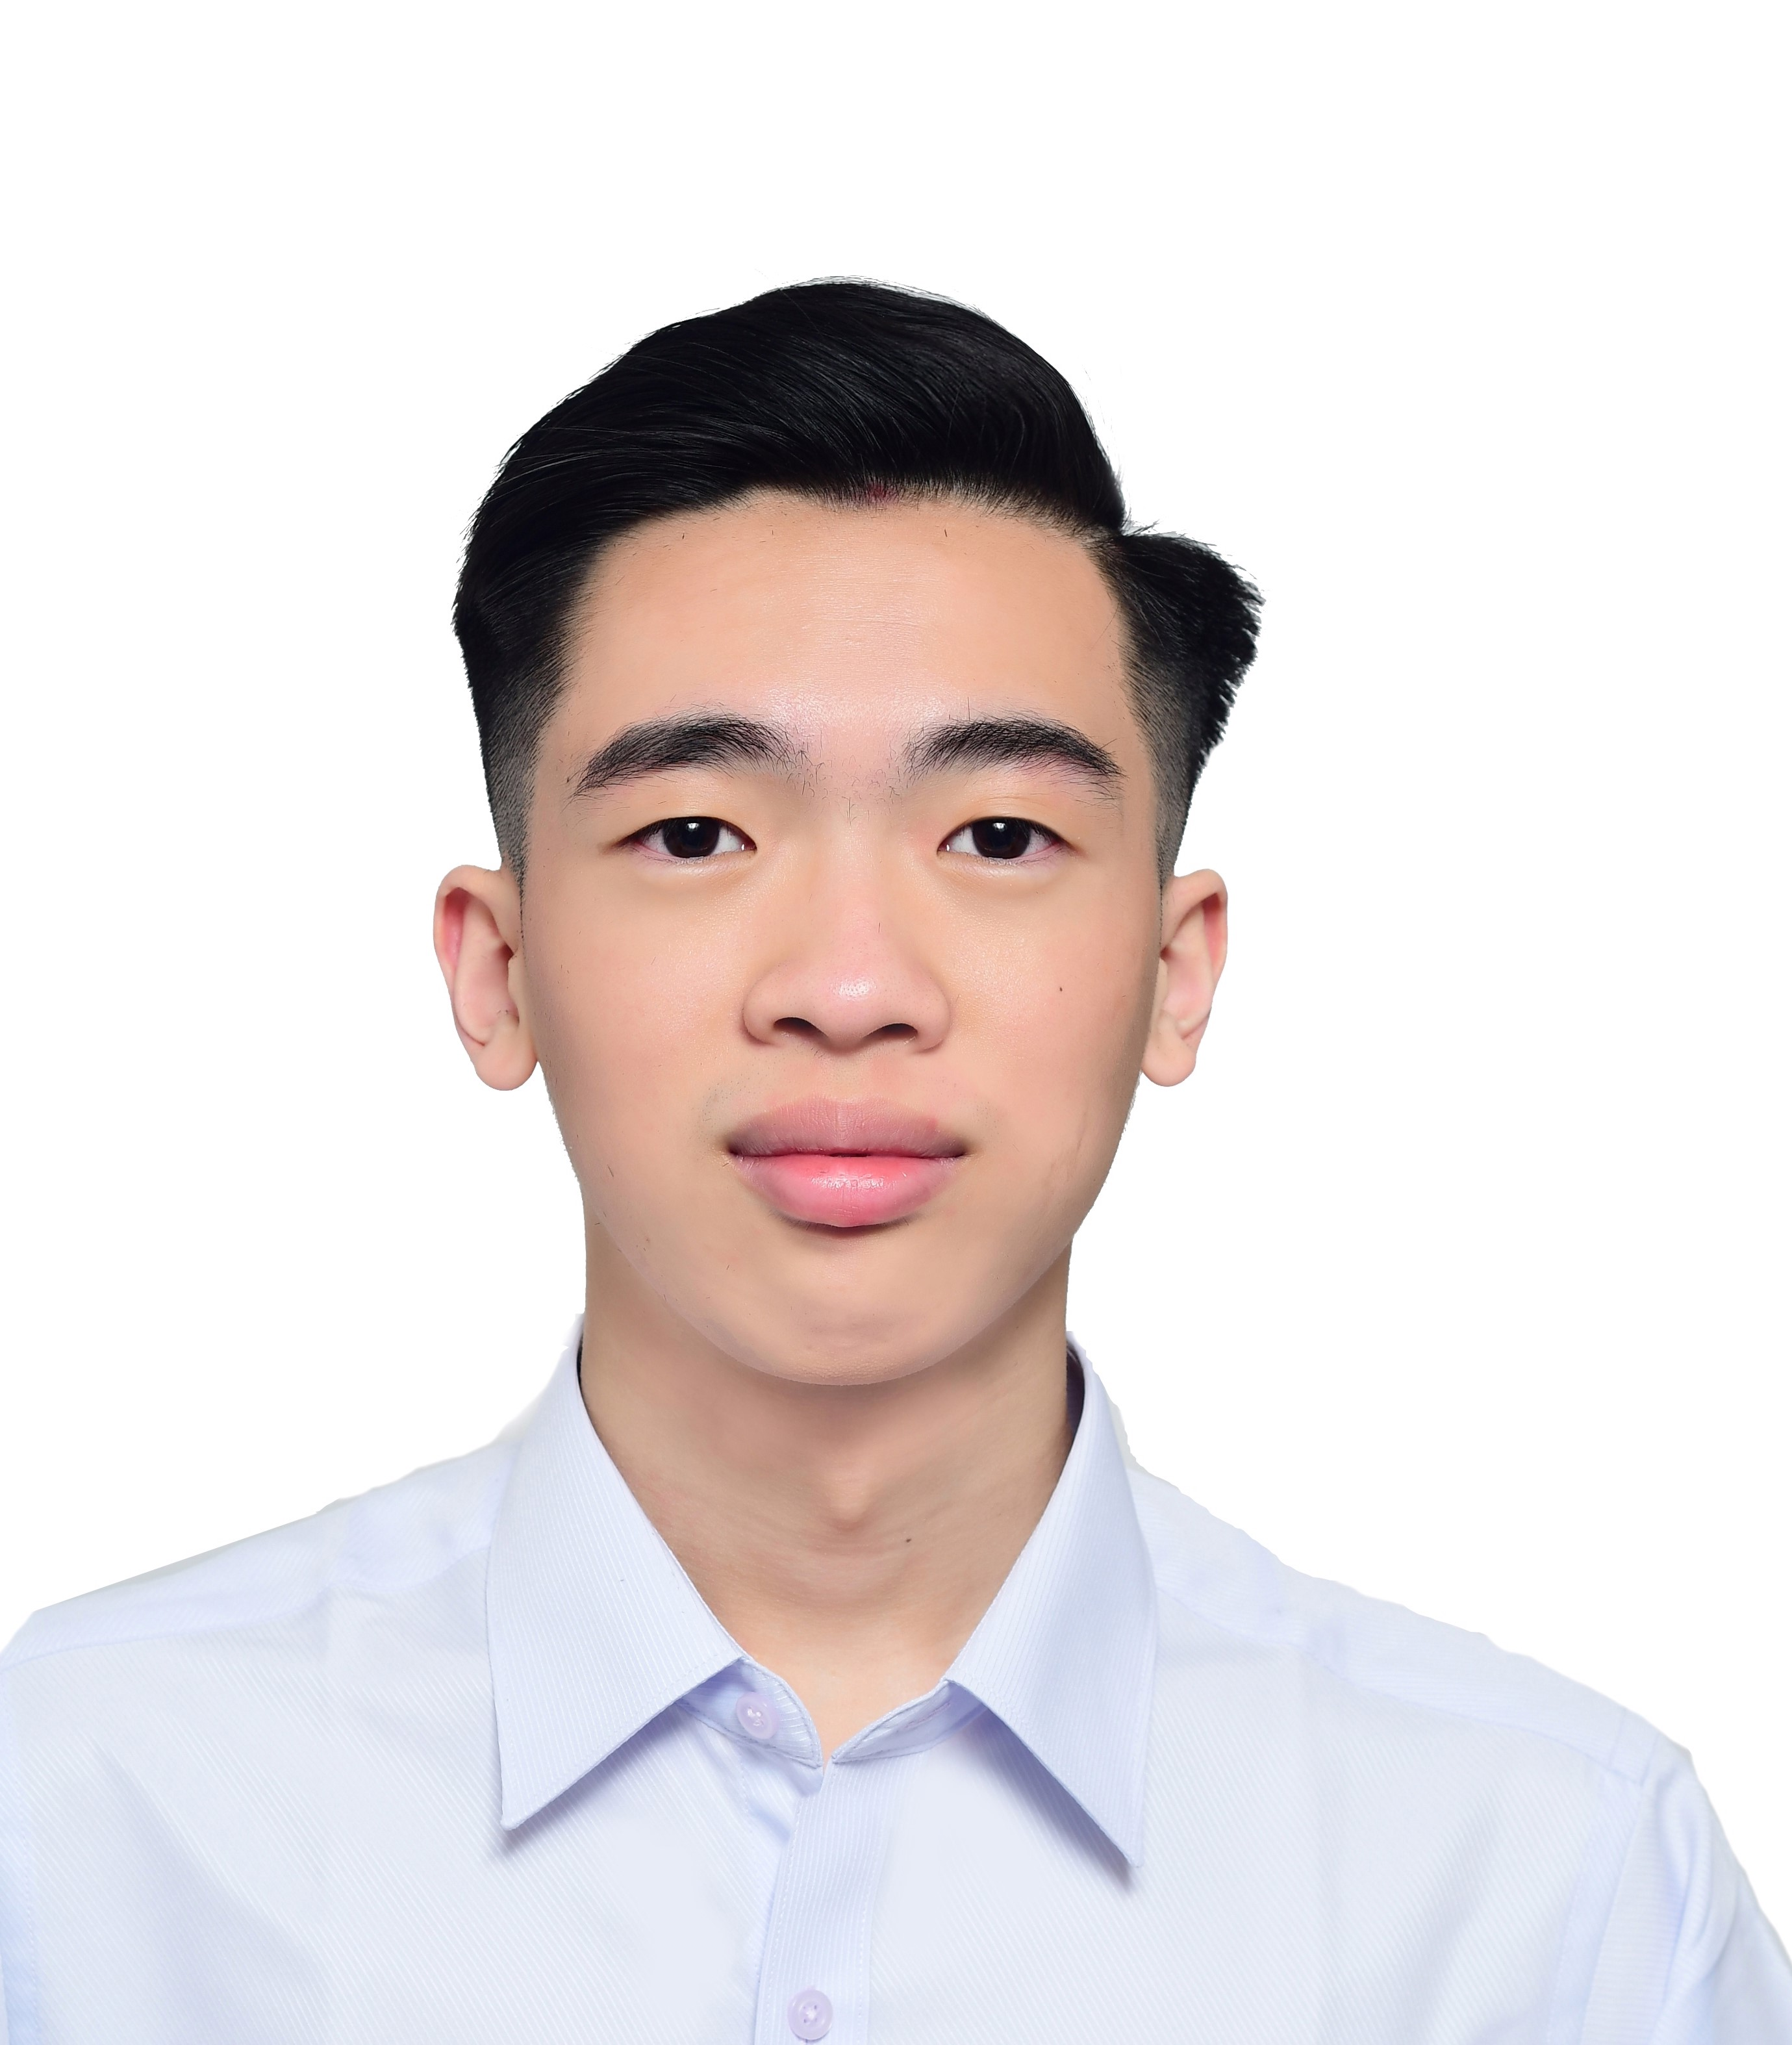
\includegraphics[width=1in,height=1.25in,clip,keepaspectratio]{picture/Chun-Mu, Weng.jpg}}]{Chun-Mu Weng}(18\%)
is currently a junior pursuing a B.S.~Degree in Computer Science at National Tsing Hua University. His interests includes but is not limited to machine learning and high-performance computing. He was responsible in doing paper research, programming, and organizing the report.
\end{IEEEbiography}

\begin{IEEEbiography}[{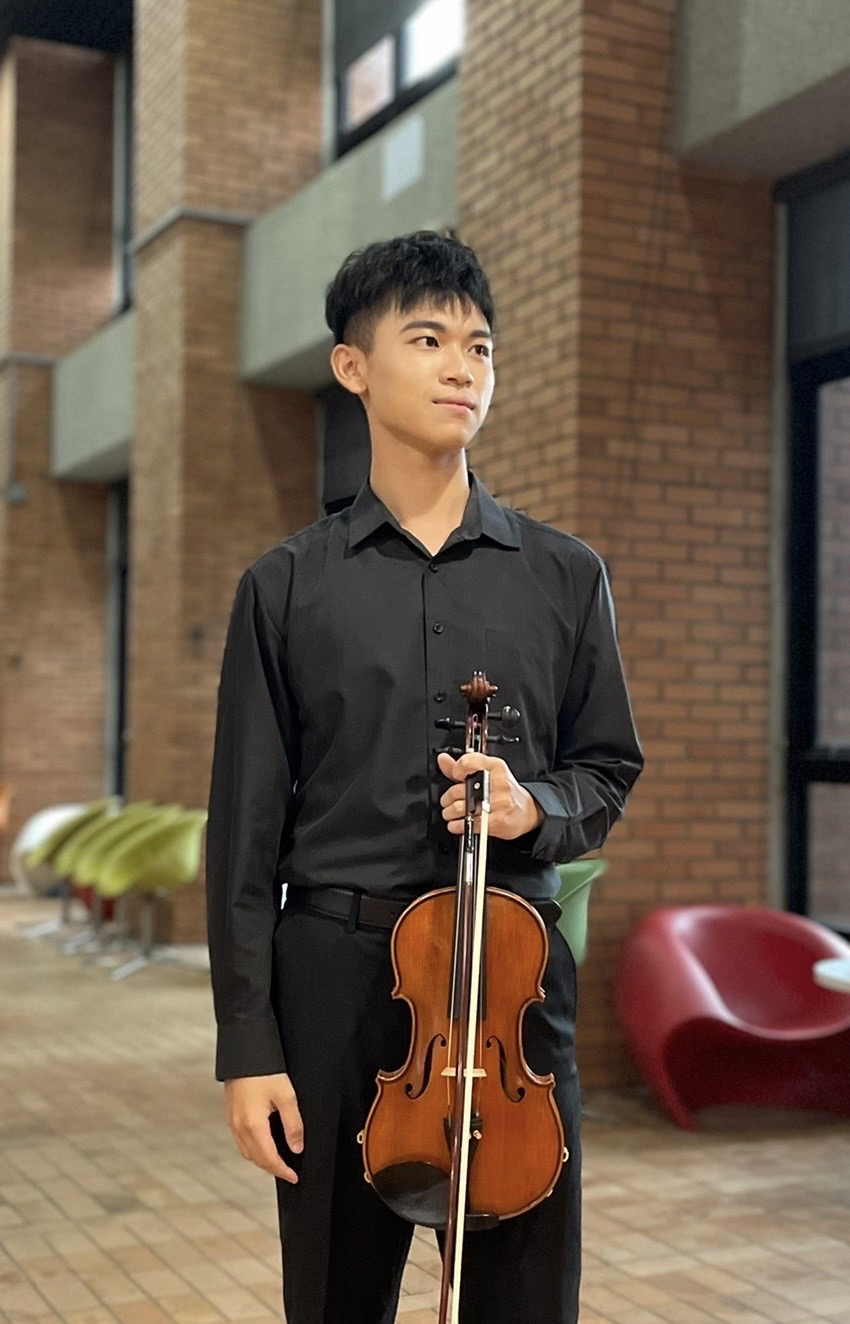
\includegraphics[width=1in,height=1.25in,clip,keepaspectratio]{picture/Ken Wu.jpg}}]{Chen-Chun Wu}(16\%)
is currently a senior majoring in Computer Science at National Tsing Hua University. His interests are extended reality and cybersecurity. For this project, he is responsible for presenting the report, organizing data of literature reviews, collecting records, and doing paper research.
\end{IEEEbiography}

\begin{IEEEbiography}[{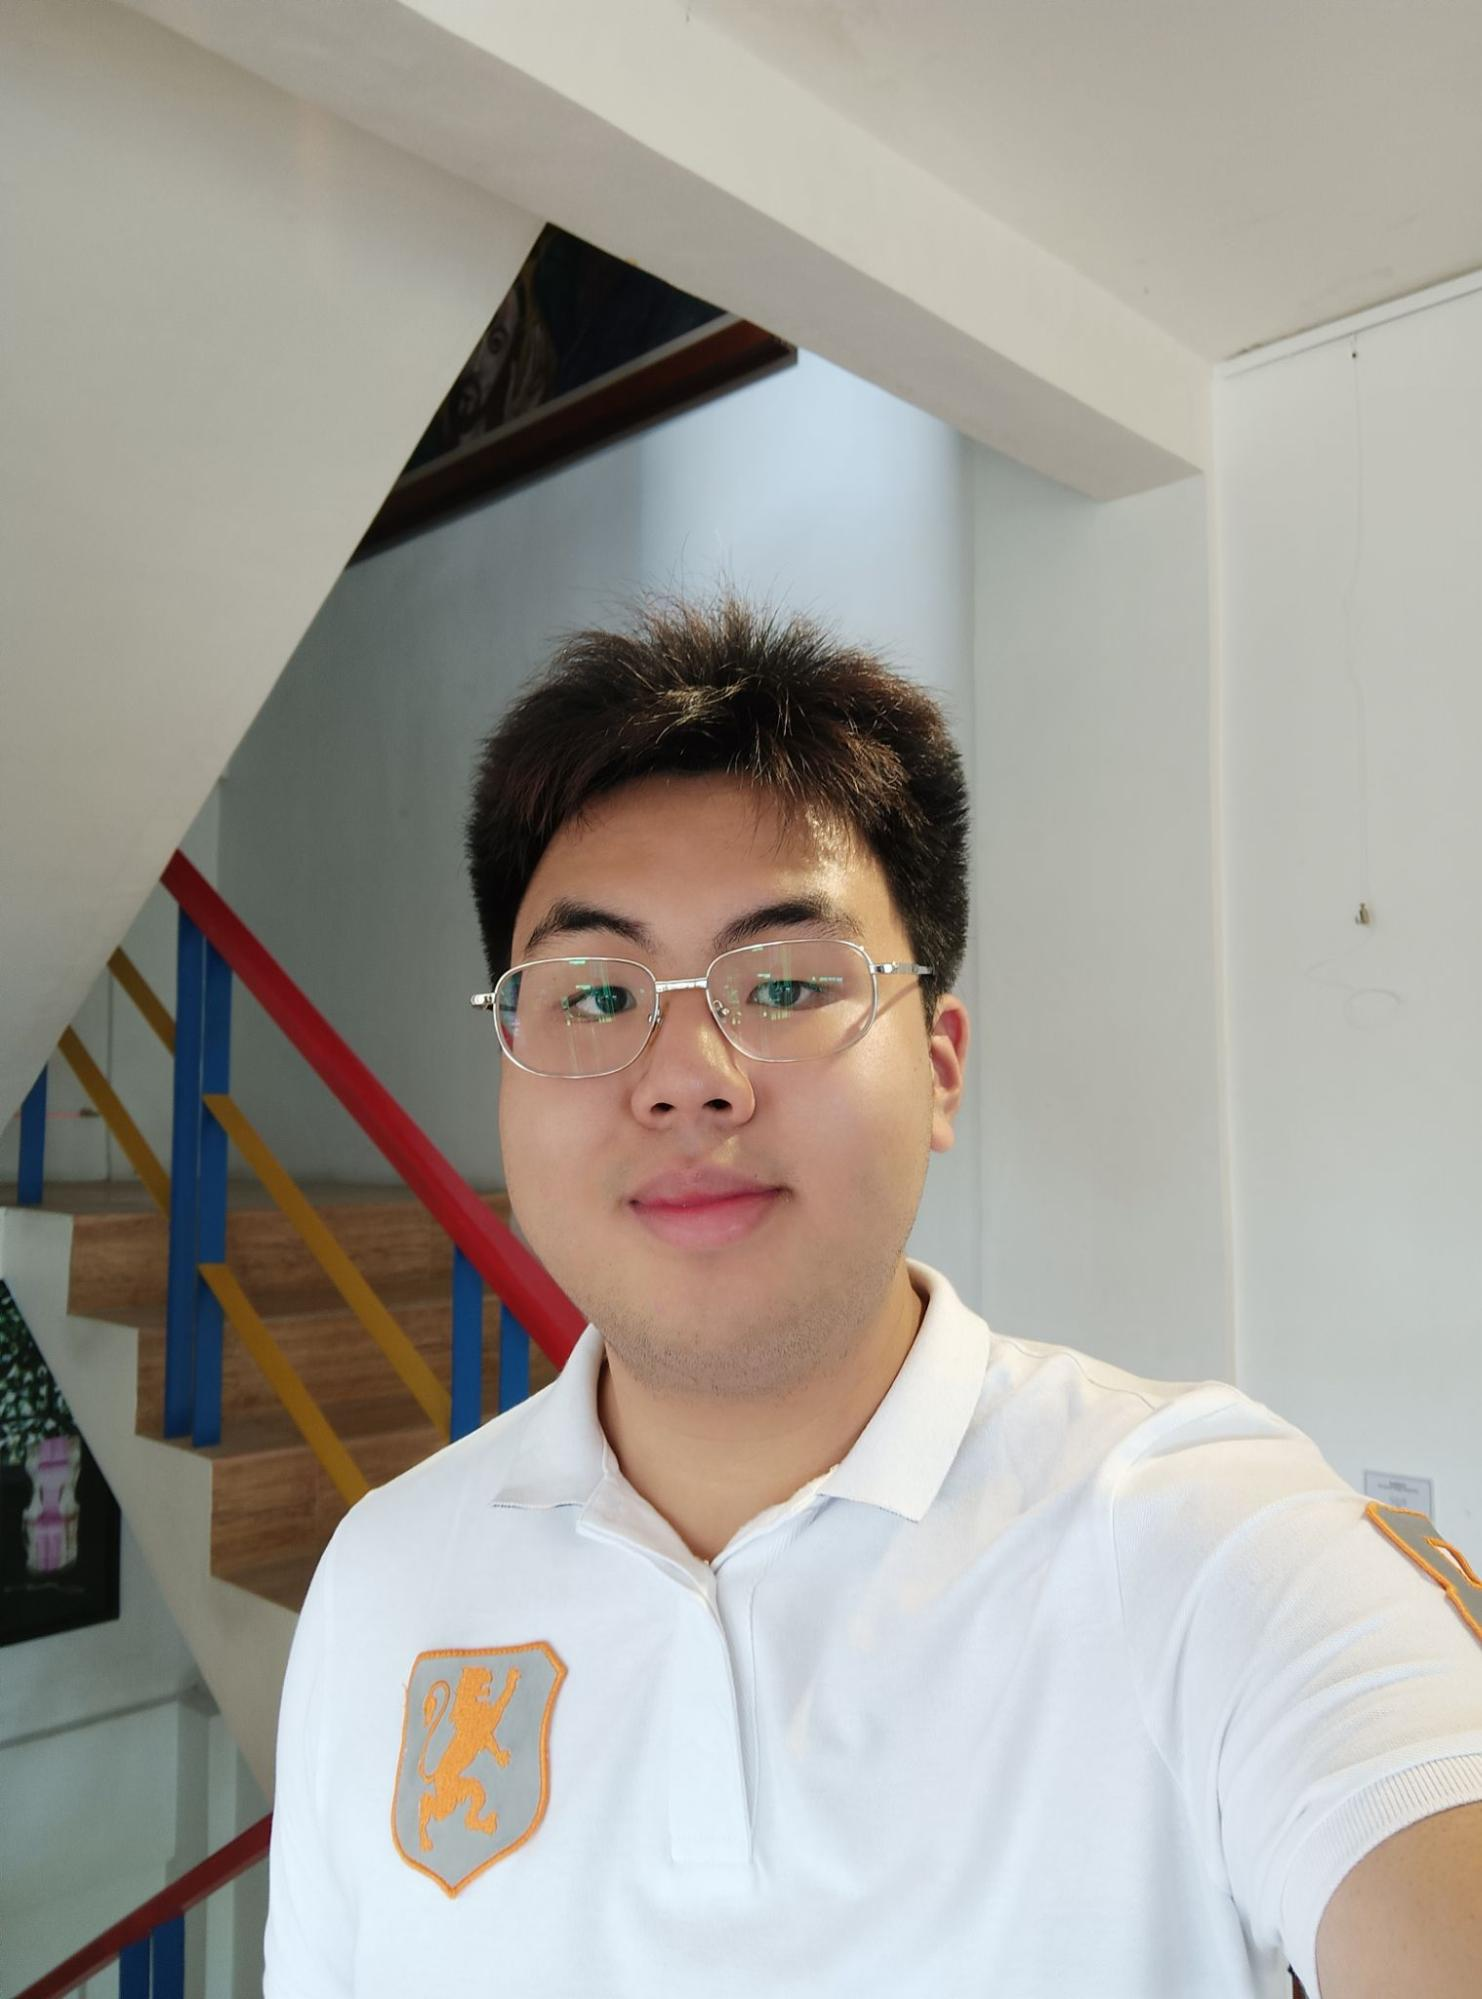
\includegraphics[width=1in,height=1.25in,clip,keepaspectratio]{picture/Jericho Hacques Michael Fajardo.jpg}}]{Jericho Jacques Michael Fajardo}(16\%)
He is currently pursuing a B.S. Degree in Electrical Engineering and Computer Science as a junior at National Tsing Hua University. His interests lie in computer vision and machine learning. He is responsible for presenting the report, organizing data from related literature, collecting records, writing the meeting minutes, and conducting paper research.
\end{IEEEbiography}

\begin{IEEEbiography}[{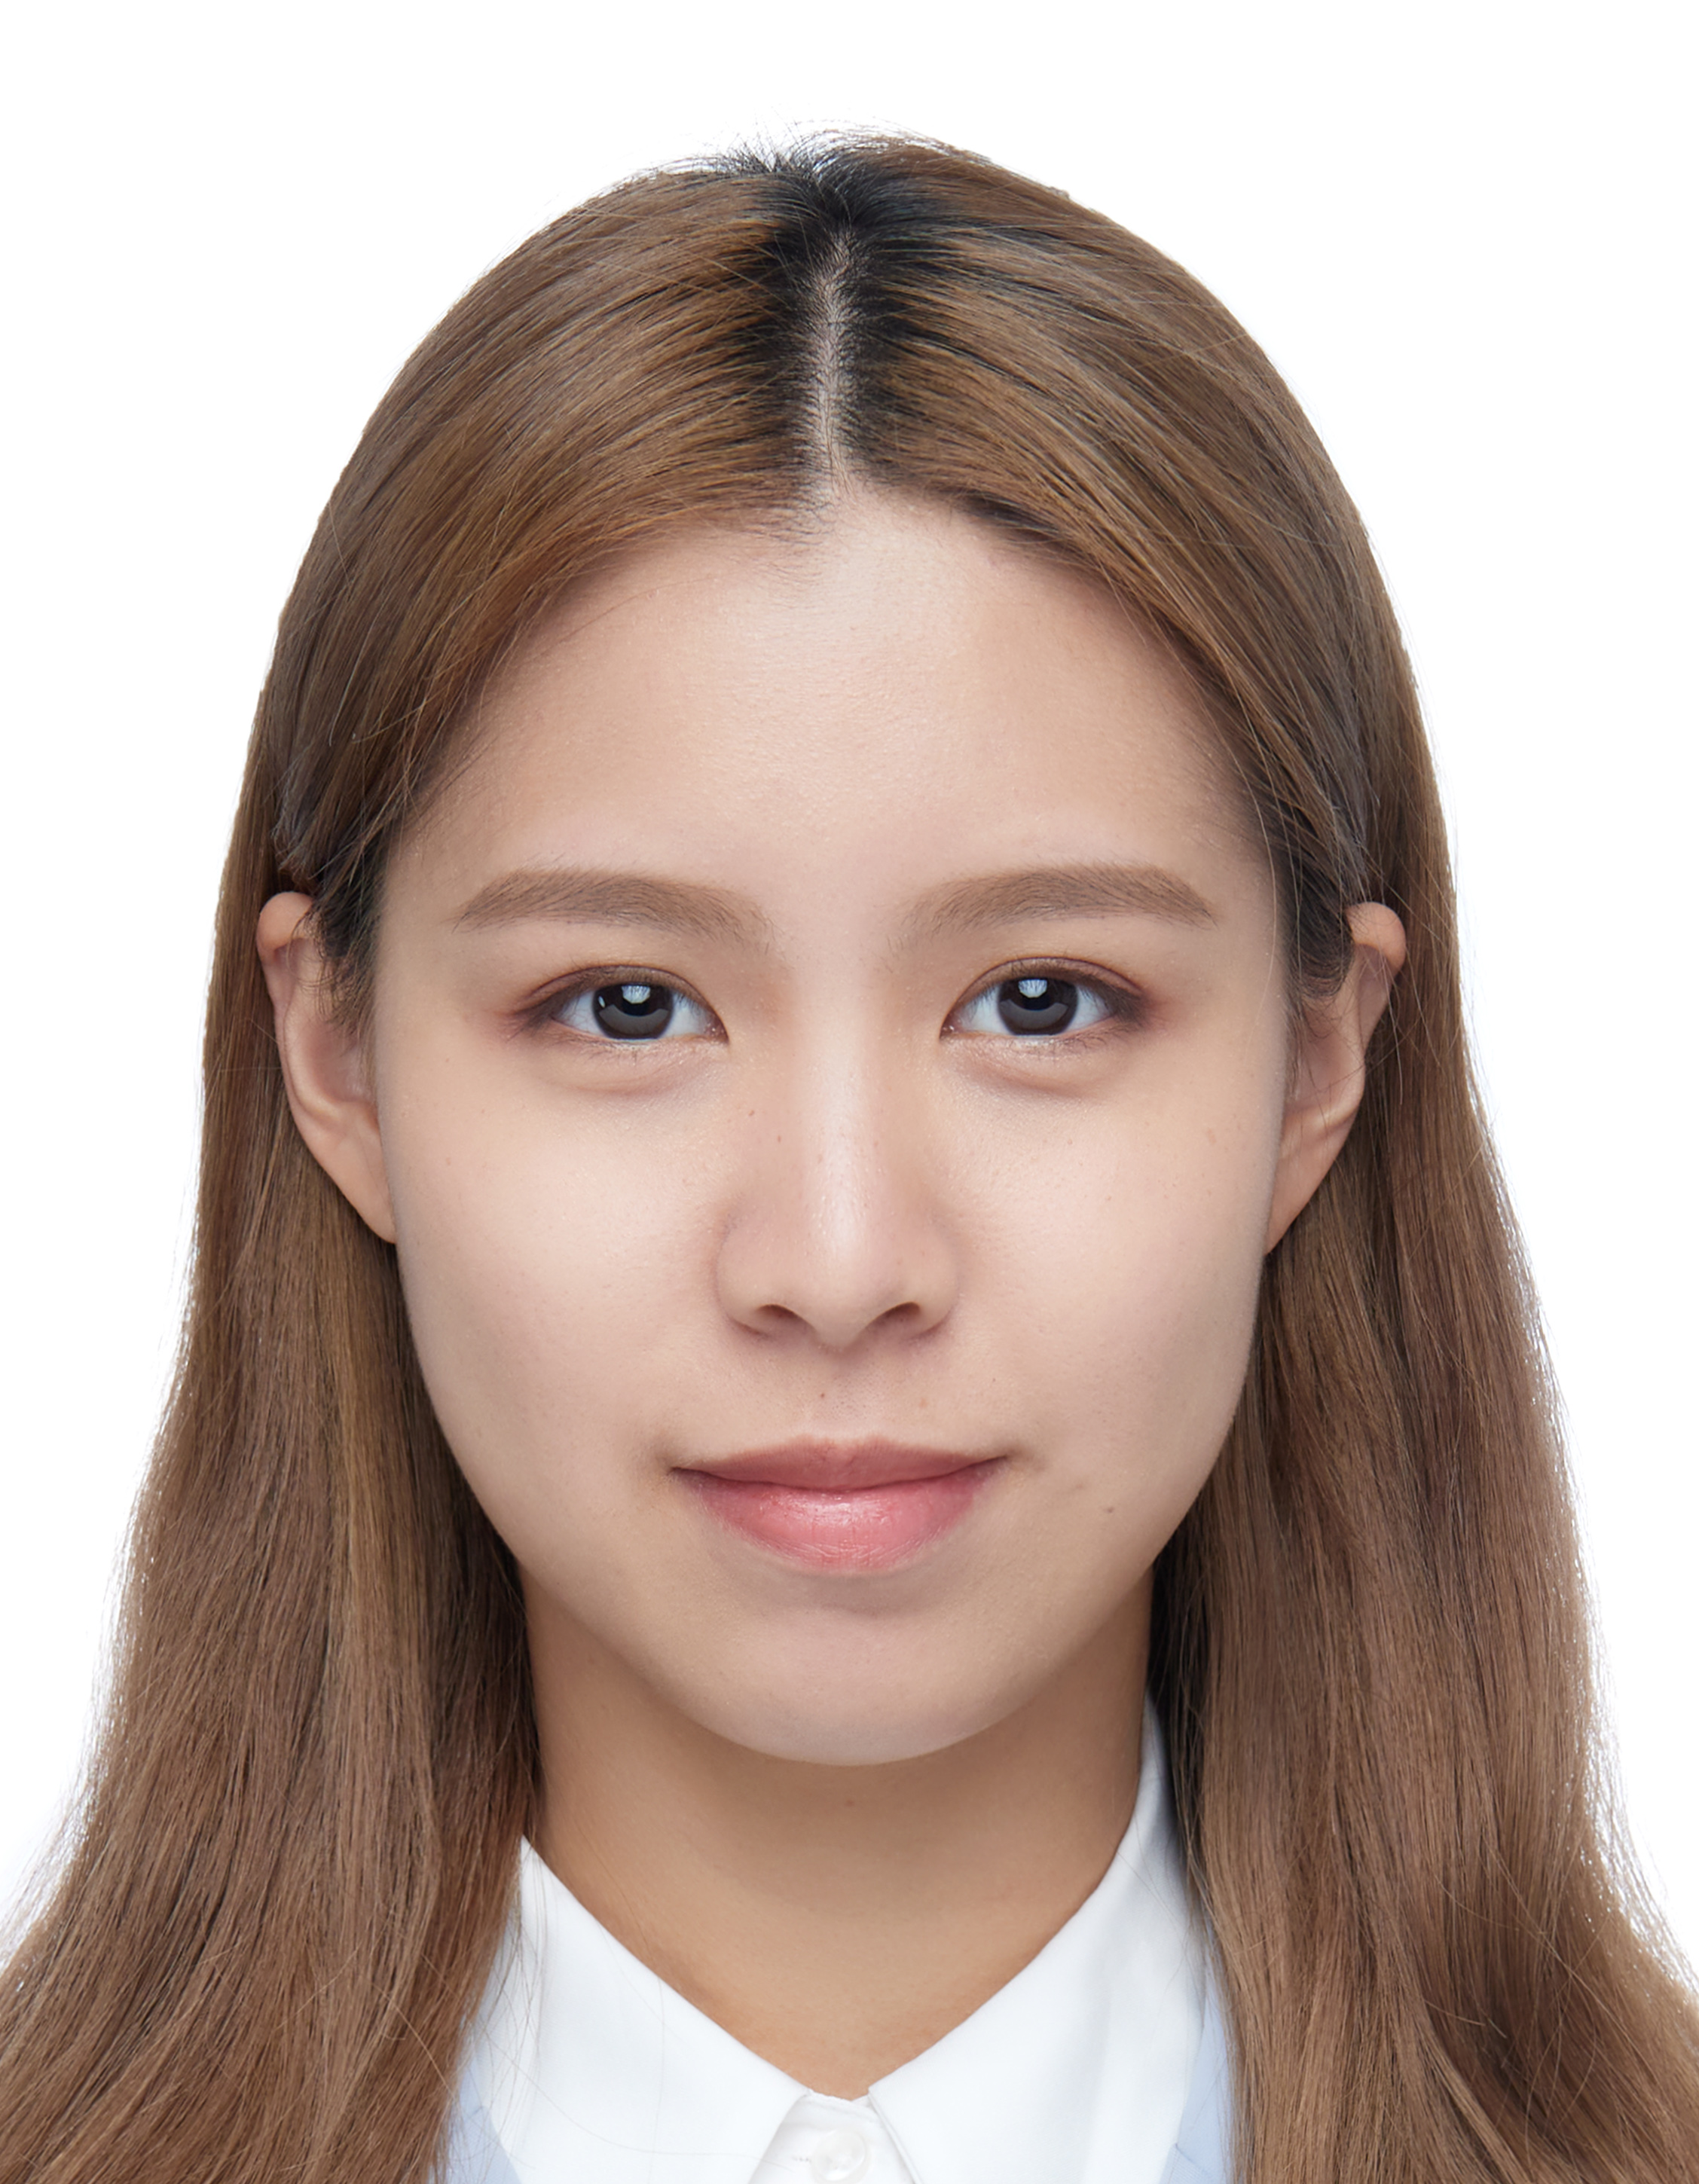
\includegraphics[width=1in,height=1.25in,clip,keepaspectratio]{picture/Shun-Han, Chang.png}}]{Shun-Han Chang}(16\%)
She is currently a junior in Department of Computer Science at National Tsing Hua University. In this project, she served as the leader and project manager, responsible for scheduling and facilitating each meeting. She also conducted paper research and organized the data for the final literature review.
\end{IEEEbiography}

\begin{IEEEbiography}[{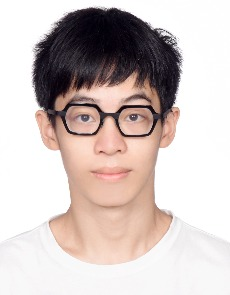
\includegraphics[width=1in,height=1.25in,clip,keepaspectratio]{picture/Tai-Hsiang, Peng.jpg}}]{Tai-Hsiang Peng}(18\%)
He is currently a junior in pursuit of a B.S.~Degree in Computer Science at National Tsing Hua University. His primary area of interest is Competitive Programming, followed by Cybersecurity. He contributed to conducting research, programming, and organizing reports.
\end{IEEEbiography}

\vspace{-155mm}

\begin{IEEEbiography}[{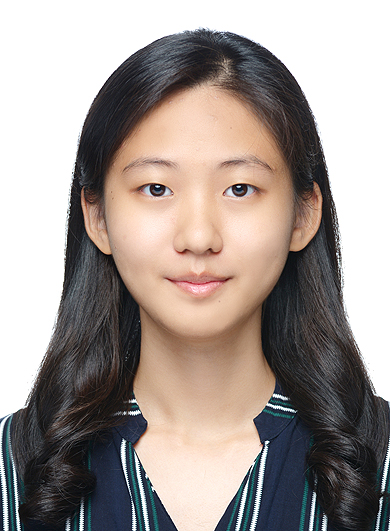
\includegraphics[width=1in,height=1.25in,clip,keepaspectratio]{picture/Ting-Yu, Lin.jpg}}]{Ting-Yu Lin}(16\%)
She studies Electrical Engineering and Computer Science at National Tsing Hua University. She conducted experiments on Linguistic models, did paper research, designed the slides, and recorded the proposal video.

\end{IEEEbiography}

% that's all folks
\end{document}
